\documentclass[a4paper,conference]{IEEEtran}
\IEEEoverridecommandlockouts
% ============ PACKAGES =============

% *** CITATION PACKAGES ***
\usepackage{cite}
% *** COMMON MATH PACKAGES ***
\usepackage{amsmath,amssymb,amsfonts}
% *** GRAPHICS RELATED PACKAGES ***
\usepackage{graphicx}
% *** TABLES RELATED PACKAGES ***
\usepackage{booktabs}
% *** PDF, URL AND HYPERLINK PACKAGES ***
\usepackage{url}
% *** SPECIALIZED LIST PACKAGES ***
\usepackage{algorithmic}
% *** SUBFIGURE PACKAGES (MANDATORY) ***
\usepackage{subcaption}
\captionsetup[figure]{name={Figure},labelsep=period, font=footnotesize}
%\captionsetup[table]{labelsep=period, font={sc,footnotesize} }

% ============ COMMANDS =============

\newcommand{\authorfont}{\fontsize{11pt}{10pt}\selectfont}
\renewcommand\IEEEkeywordsname{Keywords}

% some macros for maths
\newcommand{\bs}[1]{\boldsymbol{#1}}
\newcommand{\ma}[1]{\bs{\mathcal{#1}}}
\newcommand{\seq}[1]{\bs{#1}}
\newcommand{\set}[1]{\mathcal{#1}}

% ============ DOCUMENT STARTS HERE ============ 

\begin{document}

\title{Prototyping Cellular Command-and-Control Platform for UAS \\\vspace{10pt} }

\author{\IEEEauthorblockN{\authorfont Boris Resnick}
\IEEEauthorblockA{\normalsize Chief Technology Officer \\
\normalsize Flyvercity \\
\normalsize Netanya, Israel \\
\normalsize boris@flyver.city}
}

\maketitle

\begin{abstract}
The paper describes the basic architecture and implementation details of an edge-native platform for command-and-control of Uncrewed Aviation Systems (UAS) via a cellular network. Discovery, reliability, security, and decentralized authorization aspects are discussed.
\end{abstract}

\begin{IEEEkeywords}
UAS, drones, cellular, C2, 5G, MEC
\end{IEEEkeywords}

\section{Introduction}
Over the coming years, the use of Uncrewed Aviation Systems (UAS) a.k.a. drones will expand massively. Urban skies will become more and more packed with UAS. The number of flights and associated safety risks would increase accordingly.

A new world of product and service delivery will emerge. Most of these operations would be conducted in beyond visual line of sight (BVLOS) mode, and therefore aviation-grade reliable command-and-control link would be required. Without this critical part scaling of the industry is impossible, and therefore the global potential of air mobility market (once estimated as \$1.5 trillion \cite{market}) will remain unrealized. 

When UAS command-and-control (C2) connectivity employs a cellular network, specifically for BVLOS, there is a number of considerations for an operator to resolve. These issues are driven by required capabilities, standardization, and regulation.

While an operator may able to implement all C2 aspects by themselves, scalability requirements call for a more centralized and coordinatied approach. This is where a C2 middleware platform comes into play. Our general approach is to address this problem is defined the this paper \cite{uai}.

We identify the following aspects of C2 connectivity that need to be addressed:

\begin{itemize}
\item establish a discovery mechanism between airborne and ground entities.
\item manage reliability of connection by interacting with 5G network functions.
\item support data transmission security by managing security credentials as defined by aviation regulation \cite{icao:annex10VI} and \cite{rtca:do377a}.
\item support aerial connection authorization to address emerging regulatory requirements as defined by telecom regulation \cite{3gpp:uuaa}
\item manage remote pilot station (RPS) access to drones under control.
\end{itemize}

\section{Commmand-and-Control Middleware Platform}

This paper describes a possible approach to address the above issues. The approach is to build a platform based on the following principles:

\begin{itemize}
\item The platform is based on a cloud native architecture.
\item The platform is designed to be deployed on mobile network operator's (MNO) resources, following the concept of multi-access edge computing (MEC).
\item The implementation in open-source and extensible.
\end{itemize}

This paper describes our attempt to build such a platform, with a working title of C2NG (next-generation command-and-control).

There are two types of users of the platform:

Aerial Connection Users are flying objects comprising 5G user equipment (UE) and requiring to establish a reliable connection. Generally these are Aerial Vehicles a.k.a. drones. These also may include Wireless RPS a.k.a. ground control stations (GCS).

Aviation Data Exchange (ADX) Users are stationary entities that connect to aerial users via the ADX, but not via any 5G radio. These are generally fixed ground control center workstations.

\subsection{Discovery and Connections}

The main use case of the service is the Session Establishment procedure reflected on the following diagram:

\begin{figure}[!ht]
\centering
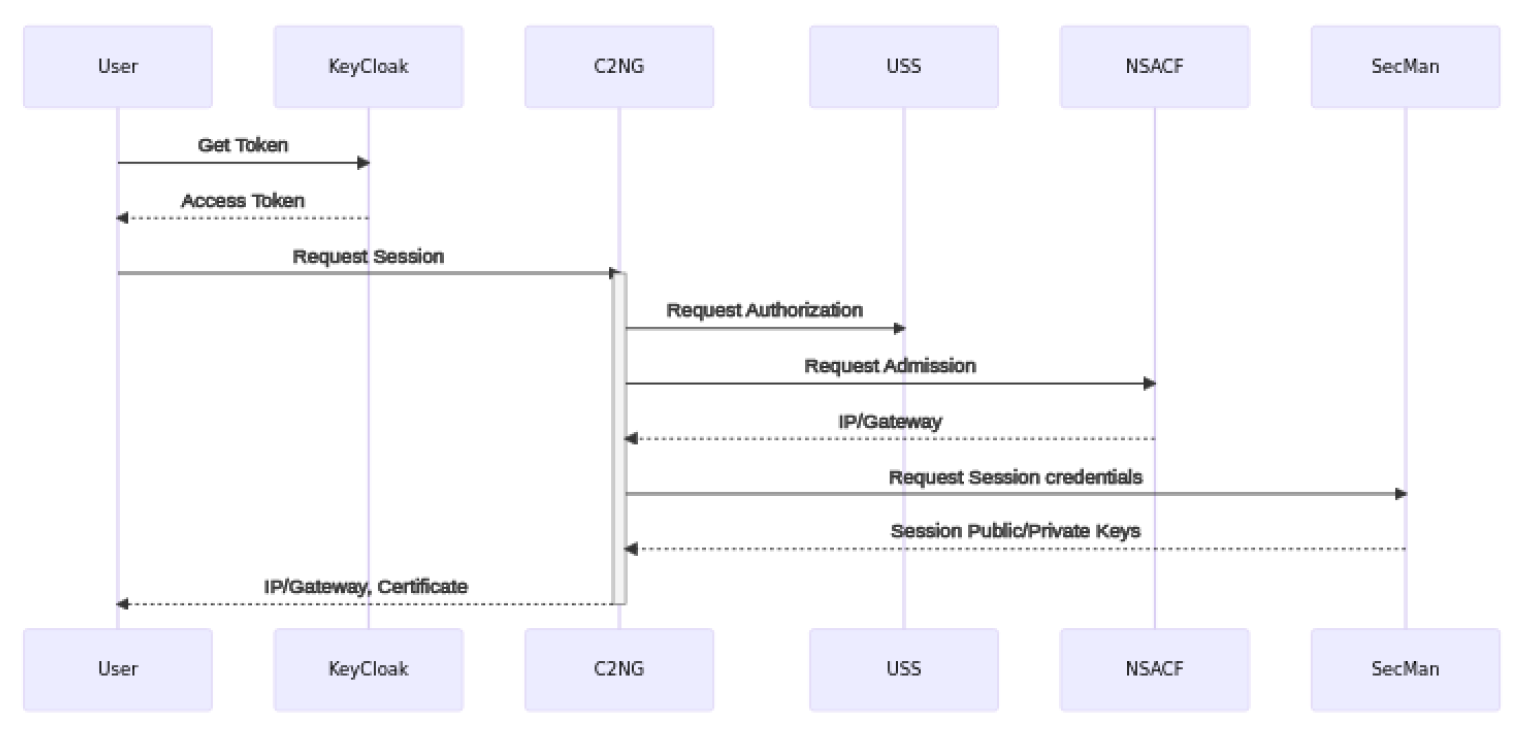
\includegraphics[width=0.9\linewidth]{images/session.png}
\caption{Session Establishment Procedure}\label{fig:session}
\end{figure}

A central concept used by the service to enable discovery procedures is Logical ID. The same uncrewed vehicle may be represented by different identification schemas, include civil aviation authority-issued identification number, internal ID of a drone operator, a designator used by Uncrewed Traffic Management (UTM) system, or 3GPP-defined identifier such as IMSI (International Mobile Subscriber Identity). The service maintains the mapping between all these identification schemas to a single Logical ID. The Logical ID is used to identify the drone, as well as the RPS, in all interactions with the service. This enables a transparent discovery procedure, where the service is able to identify the drone and its RPS, regardless of the identification schema used by the drone operator.

Main flow on the connection procedure supported by the service is as follows:

\begin{enumerate}
\item The drone requests a connection session by providing the Logical ID of the drone and the RPS.
\item The service performs lookup of the relevant drone and RPS identifiers by the Logical IDs.
\item The service creates a connection session.
\item Network management subsystem select a proper MNO and ADX, and ensures that network quality of service configuration is relevant to the session requirements.
\item The service request an authorization from the relevant UTM system and supports the authorization procedure, which will be initiated by the 5G network \ref{uuaa}.
\item The service creates session security credentials (\ref{security}) and provides them to the drone and the RPS together with the connection parameters.
\end{enumerate}

This procedure enables truly dynamic discovery and connection procedures, where the drone operator is not required to pre-register the drone with the RPS and vice versa. The service is able to identify the drone and the RPS by the Logical ID, and the drone operator is able to use any identification schema they prefer.

\subsection{Reliability}

The primary goal of the service is to ensure reliable connectivity between the drone and the RPS. The service is able to achieve this goal by interacting with the 5G network functions. First of all, the service is able to request a specific network slice to be allocated to the session. The service is also able to request a specific quality of service (QoS) configuration.

For the perspective of the requested drone operation, the QoS is determined by the following parameters (RLP - Required Link Performance as defined by \cite{rtca:do377a}).

{\b Availability} is minimum percentage of time that the services of the system are usable with the level of guarantee on latency and throughput.

{\b Continuity} is an acceptable probability of a successful delivery of a message after its transmission was started assuming the communications system is available when the transmission is initiated. Any error that can be corrected on a transport level or below is not included here.

{\b Integrity} is an acceptable probability of elementary message transmission was completed with an undetected error. Error is detected if sending party receives a timely (within latency time) notification from Data Transmission Service. Loss of integrity includes a risk of data corruption due to tampering and other possible security issues.

An external user, such as a drone operator, is not able to determine a mapping between these parameters and network configuration. On the contrary, the service, being tightly integrated with the network, can derive feasibility of QoS provision and necessary measures.

For the cellular implementation, the integrity parameter is driven by a probability of data corruption. Assuming sane and correct checksum-based procedures are in place, probability of integrity loss as associated with a probability of intentional data tampering. The service addresses this issue by providing session security credentials. The user, however, is responsible for the correct implementation of the encryption and signing procedures \ref{security}.

Parameters controlled by the network may vary depending on the given network architecture. During our trials, we used a multi-step procedure:

\begin{enumerate}
\item RLP parameters looked up in the database based on the drone type and the requested operation.
\item Based on Availability/Continuity requirements, the service selected one of a set pre-configured network slices.
\item The slice's 5QI (5G QoS Identifier) was adjusted based on latency requirement (see \cite{3gpp:rely}).
\item Overall throughput is analysed to avoid any overloads.
\item New user (aerial or an ADX) was added to the slice via the NSACF.
\end{enumerate}

It is also worth mentioning that these technical provisions should be supported by organizational means such as SLA (Service Level Agreements) when deployed operationally.

\subsection{Security}
\label{security}

Cellular radio communications are inherently secured by 3GPP-defined mechanisms. Nevertheless, the regulation also calls for end-to-end reliable encryption. To support this requirement, the platform implements session security credentials management based by asymmetric cryptograhy. This prototype supports RSA encryption (\ref{section:keys}). It is also important for all participants to apply the protocol correctly as described in \ref{section:exchange}. An additional security mechanism associated with RPS access to drones is described in \ref{section:did}.

\subsubsection{Key Management}
\label{section:keys}

The service uses a static root private key and a corresponding certificate to sign a user session certificate, hence serving as a local cerfication authority (see Figure \ref{fig:keys}). A new session key pairs are generated upon creation of the session, separately for aerial and ground users. 

\begin{figure}[!ht]
\centering
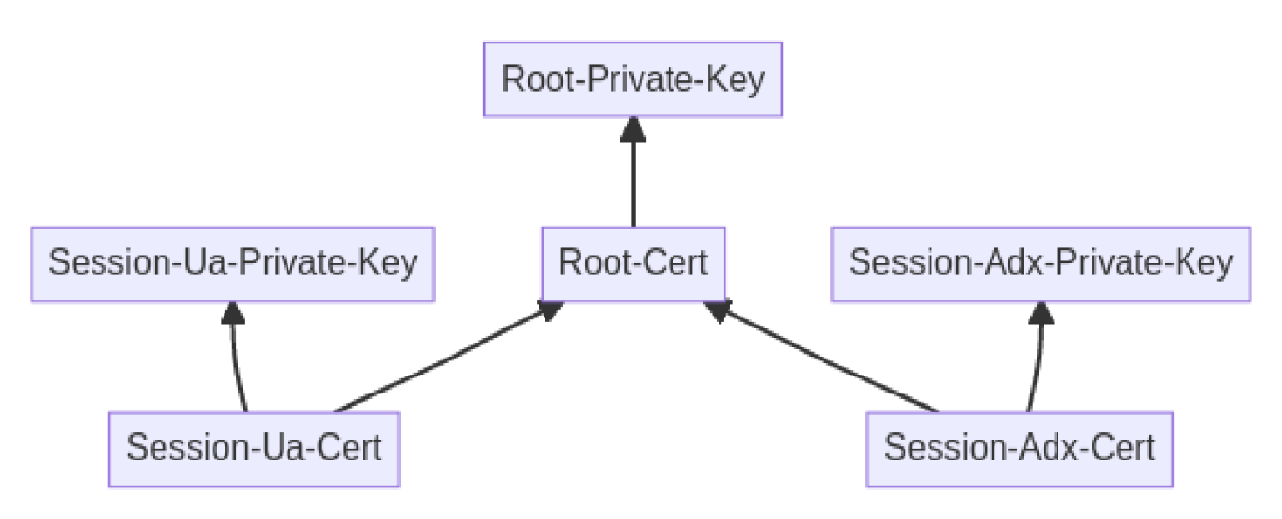
\includegraphics[width=0.9\linewidth]{images/keys.png}
\caption{Keys Hierarchyl}\label{fig:keys}
\end{figure}

Public keys are distributed to the users during the discovery and session identification procedure.

\subsubsection{Secure Data Exchange Procedure}
\label{section:exchange}

Correct key distribution is not enough to ensure integrity. Below is a standard procedure that is obligatory for all users to follow to ensure secure data exchange (see Figure \ref{fig:exchange}).

\begin{figure}[!ht]
\centering
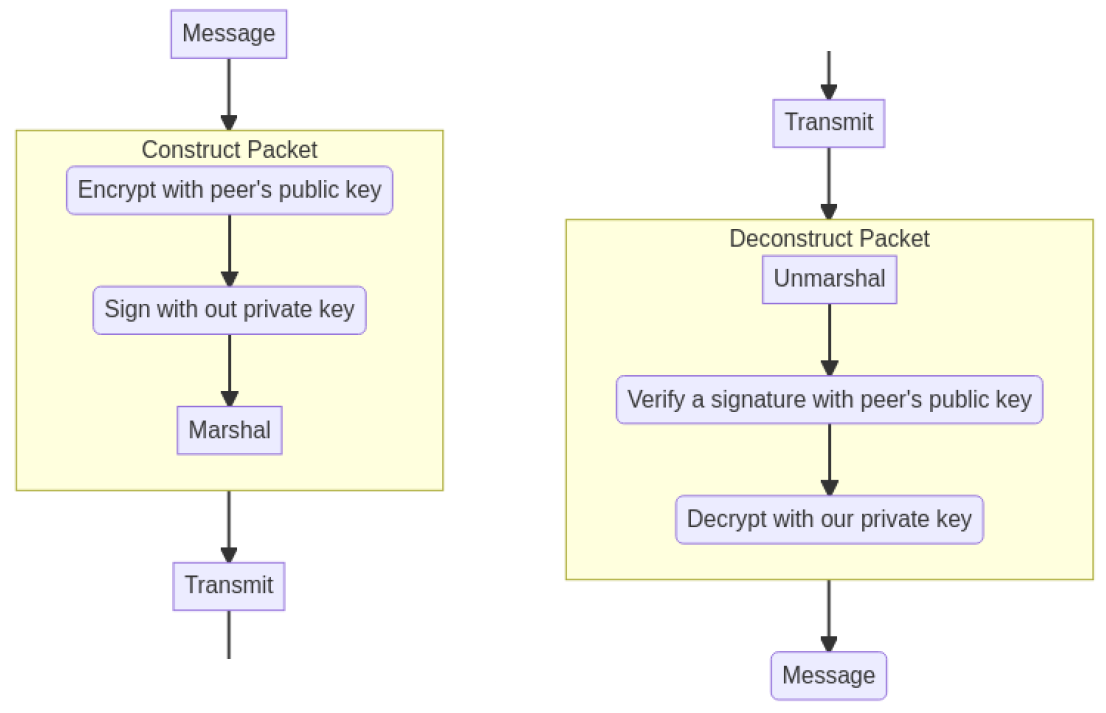
\includegraphics[width=0.9\linewidth]{images/exchange.png}
\caption{Session Establishment Procedure}\label{fig:exchange}
\end{figure}

It shall be noted, that for the sake of simplicity, the figure does not show any procedures required to transmit longer messages (e.g., see \cite{cryptoeprint:2000/065}). 

\subsection{Aerial Connection Authorization}
\label{uuaa}

The platform supports the USS (UTM Service Supplier) UAV (Uncrewed Aerial Vehicle) Authorization and Authentication (UUAA in 3GPP terminology) procedure as defined by \cite{3gpp:uuaa}. 

\begin{figure}[!ht]
\centering
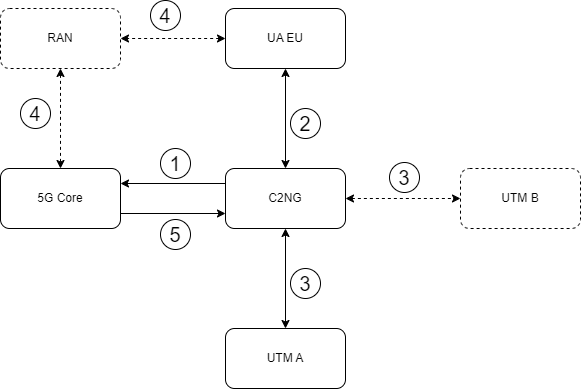
\includegraphics[width=0.9\linewidth]{images/uuaa.png}
\caption{USS UAV Authorization and Authentication}\label{fig:uuaa}
\end{figure}

This procedure involves several entities and steps:

\begin{enumerate}
  \item The platform registers itself within the Core as entity responsible for UUAA.
  \item The drone requests a connection session from the platform.
  \item The platform determines relevant UTM system(s) based on flight intent provided by the drone, and requests authorization from the UTM system(s).
  \item The drone's cellular user equipment (UE) requests a connection. This connection is identified by the 5G System as aerial based on the UE identification.
  \item This request triggers the UUAA procedure. The 5G Core requests the platform to provide the authorization data.
\end{enumerate}

Hence, in the presence of the C2NG platform, neither drone nor UTM system are required to implement any specific procedures to support UUAA. The platform is able to support any UTM system that is able to provide the authorization data.

\subsection{Remote Pilot Station Access}
\label{section:did}

To help drone operators (designated in this section as "owners") manage their fleet, the platform provides a mechanism to manage access to the drones by remote pilot stations (RPS).

\begin{figure}[!ht]
\centering
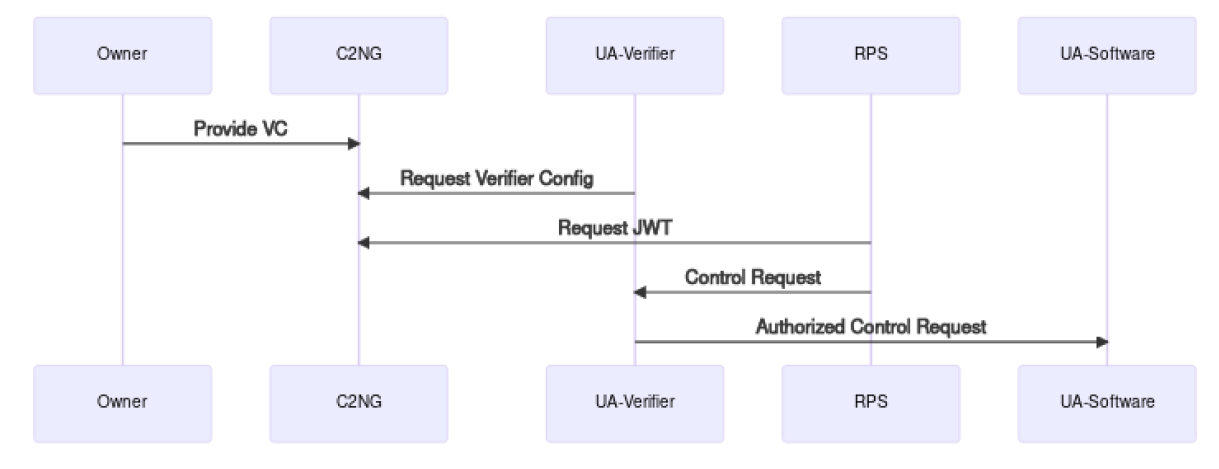
\includegraphics[width=0.9\linewidth]{images/did.png}
\caption{Decentralized Identification}\label{fig:did}
\end{figure}

The platform supports remote pilot station authorization to control the drones via the advanced decentralized identification mechanism \cite{excid:did}. The DID solution provides the Verified Credentials mechanism which allows the platform or its users to manage authorization without permanent connection to the drones or the pilot stations themselves.

The platform supports the following "key" and "self" DID types, and can serve as a drone owner or support drone operator as an owner. For purposes of the decentralized authentication mechanism, the "owner" is an entity that issues a verifiable credential to their RPS station under control.

A drone itself implemements a verifier that operates based on the verifier configuration provided by the platform. The verifier is able to determine if the RPS is authorized to control the drone, based on the encrypted token provided by the RPS.

\section{Implementation and Evaluation}

This section describes the implementation of the platform and some results of validation conducted in the scope of current paper's development.

\subsection{Application Architecture}

The Application is based on containerized services and comprises three open source basic components (KeyCloak, MongoDB, and InfluxDB) and the core software service (C2NG). Besides the core software, CLI (command line interface) tools were developed to control all administrative tasks, simulation, and demostration. KeyCloak is an open source implementation of the OIDC (Open ID Direct Connect) protocol and supports authorized calls to the service.

\begin{figure}[!ht]
\centering
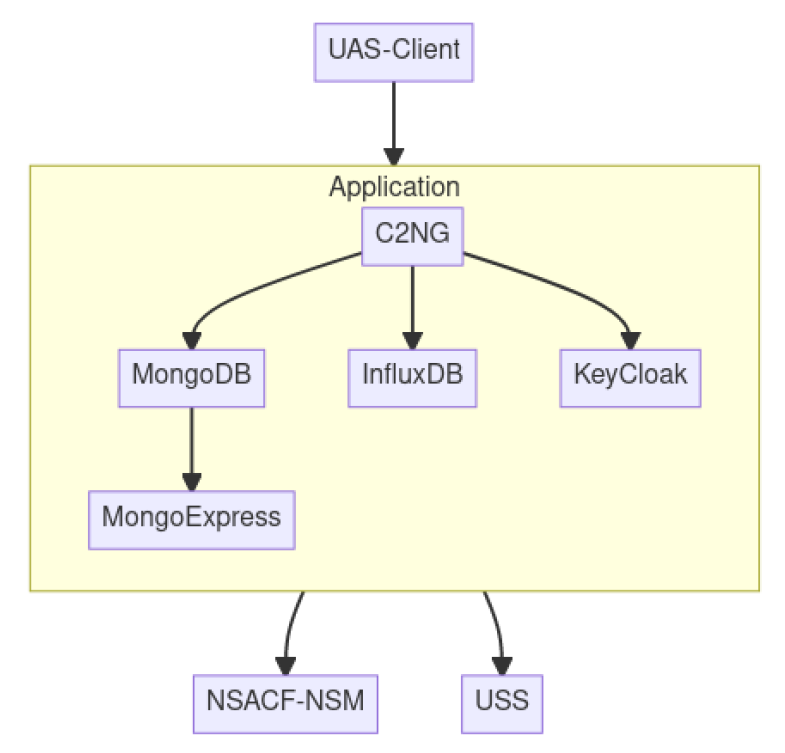
\includegraphics[width=0.9\linewidth]{images/arch.png}
\caption{Decentralized Identification}\label{fig:arch}
\end{figure}

NSACF (Network Slice Admission Control Function) is a Network Function exposed by the 5G Core to control which users are authorized to use a slice and hence enjoy high reliability allocated with it. It can be also extended by a particular implementation to control 5G slices in a more fine-grained manner (the umbrella term for this is “Network Slice Management” --- NSM).

MongoDB is a NoSQL database that serves as a persistence layer. InfluxDB is a timeseries database used to collect signal characteristics reported by aerial users. C2NG designates the service itself. C2NG is a web service and exposes two APIs. The REST API described in the API Definition section is used by the users to request connectivity sessions and report signal quality information. The second API is any web-socket based asynchronious API used to notify the users about the changes in the session status in real time.

The whole application is a set of Docker containers defined by the Docker Compose Specification for developement and single-node environments.

\subsection{Validation}

Network integration and the quality-of-service subsystem were tested in the lab, associated with the IoT-NGIN project, with an advanced 5G core that is capable of managing the network slices and providing the required connectivity for the drones.

In order to access connectivity quality, the round-trip time (RTT) metric was measured. The RTT is the time it takes for a signal to be sent plus the time it takes for an acknowledgement of that signal to be received. The RTT is measured in milliseconds (ms). The RTT was measured by the UA (uncrewed aircraft) software simulator. Two types of RTT measurements were performed: pure and encryption-aware. Pure RTT is measured based on the time required to transmit small UDP packets. Encryption-aware RTT is measured based on the time required to transmit encrypted and signed UDP (User Datagram Protocol) packets, and also to validate access tokens. The encryption is performed by both UA and RPS C2 simulators.

The results show significant, but not critical, increase in RTT when encryption is enabled. The average RTT is 5 ms (lab network) when encryption is disabled and 12 ms when encryption is enabled (given the hardware used - Core i5 laptop). The RTT is expected to be higher when the C2 software component is deployed on a real UA.

\section{Conclusion}

\begin{itemize}
\item Flyvercity C2NG Platform can be used to provide UA C2 services over 5G networks, without requiring network-operator-specific pre-flight network configuration on the UA or RPS;
\item C2NG Platform can be integrated with Verifiable Credentials components to provide a secure and privacy-preserving RPS authentication and authorization mechanism.
\end{itemize}

\section*{Acknowledgment}

This paper is based on the results of IoT UAS C2 project, a sub-project funded via the IoT-NGIN project Open Call. IoT-NGIN has received funding from the European Union’s Horizon 2020 research and innovation programme (Grant Agreement No 957246).

\begin{thebibliography}{2}

\bibitem{uai}
B. Resnick, \emph{Scaling cellular command-and-control capability for multiple drone operations},\hskip 1em plus 0.5em minus 0.4em\relax https://www.unmannedairspace.info/commentary/scaling-cellular-command-and-control-capability-for-multiple-drone-operations/, 2023. 

\bibitem{excid:did}
N. Fotiou, V. A. Siris, G. C. Polyzos, Y. Kortesniemi, D. Lagutin, \emph{Capabilities-based access control for IoT devices using Verifiable Credentials", in IEEE Symposium on Security and Privacy Workshops},\hskip 1em plus 0.5em minus 0.4em\relax Workshop on the Internet of Safe Things (SafeThings), 2022

\bibitem{3gpp:rely}
3GPP, \emph{5G; Service requirements for the 5G system}.\hskip 1em plus 0.5em minus 0.4em\relax (3GPP TS 22.261 version 16.14.0 Release 16.

\bibitem{3gpp:uuaa}
3GPP, \emph{5G; Security aspects of Uncrewed Aerial Systems (UAS)}.\hskip 1em plus 0.5em minus 0.4em\relax 3GPP TS 33.256 version 17.0.0 Release 17.

\bibitem{market}
Levitate Captital, \emph{The Future of the Drone Economy}. Whitepaper\hskip 1em plus 0.5em minus 0.4em\relax https://levitatecap.com/levitate/wp-content/uploads/2020/12/Levitate-Capital-White-Paper.pdf, 2020

\bibitem{icao:annex10VI}
ICAO, \emph{Aeronautical Telecommunications. Communication Systems and Procedures Relating to Remotely Piloted Aircraft Systems C2 Link},\hskip 1em plus 0.5em minus 0.4em\relax Annex 10 on the Convention on International Civil Aviation. 1st Edition, July 2021.

\bibitem{cryptoeprint:2000/065}
M.~Mitomo and K.~Kurosawa, \emph{How to Encrypt Long Messages without Large Size Symmetric/Asymmetric Encryption Schemes}, Cryptology ePrint Archive, Paper 2000/065.\hskip 1em plus 0.5em minus 0.4em\relax https://eprint.iacr.org/2000/065, 2000.

\bibitem{rtca:do377a}
RTCA, \emph{Minimum Aviation System Performance Standards for C2 Link Systems Supporting Operations of Unmanned Aircraft Systems in U.S. Airspace},\hskip 1em plus 0.5em minus 0.4em\relax RTCA DO-377A, 2021.

\end{thebibliography}
\end{document}